\section{Design für Analphabeten}

Beim Design für Analphabeten gibt es einige Ansätze, wie man Dinge wie bspw. Software gestalten kann, damit auch Menschen, die nicht lesen und schreiben können, diese Dinge verwenden können.\\
Hierbei ist es natürlich wichtig herauszufinden, wie diese Menschen Dinge wahrnehmen auffassen und wie ihre Herangehensweise beim erlernen neuer Dinge ist. Um dies herauszufinden ist es unter anderem in erster Linie wichtig Studien abrufen zu können, in denen soetwas bereits gemacht wurde. Dabei muss man in den meisten Fällen jedoch auf Studien zurückgreifen, die sich mit primärem Analphabetismus auseinandersetzen, da diese Studien in den meisten Fällen in Indien und den Phillipinen gemacht wurden, bei Menschen, die das Lesen und Schreiben niemals erlernt haben. Aber auch diese werden vorraussichtlich ähnliche Methoden wie funktionale Analphabeten verwenden um zu lernen.\\
Der erste schritt ist sich klar zu machen, dass die Kommunikationsschnittstelle schlecht hin nicht verwendet werden kann. Entsprechend muss das Interface für Analphabeten anders gestaltet werden. Aber fragt man sich, welche Möglichkeiten da noch in Frage kommen? Die naheliegendste Lösung wäre ein Inerface, dass die Menschen akkustisch anleitet, was zu tun ist. Sowas ist jedoch manchmal schwierig, denn Audiodateien benötigen viel Speicherplatz und möchte man bspw. ein Handy so gestalten, dass auch Analphabeten es benutzen können, so wird der Speicherplatz hier knapp für ein reines Toninterface. Daher sind viele Firmen dazu übergegangen - besonders bei Handys - das Interface mit möglichst wenig Text und mit speziell ausgewählten Bildern zu gestalten, deren Bedeutung leicht zu identifizieren sein soll.\\
Um genau zu bestimmen welche Anforderungen ein Design zu bestimmen hat, ist es von Nöten, dass kontinuierlich mit Probanden zusammen gearbeitet wird, die die bisherige Arbeit beurteilen können und den Entwicklern zeigen, an welchen Stellen sie das Design noch nicht soweit getroffen haben, dass ihre Schnittstelle einfach zu verstehen ist. Um zusätzlich zu gewährleisten, das hier ein vernünftiges doch abstraktes Ergebnis erscheint, müssen die Probanden zu jedem Test wechseln und die neuen Probanden müssen es schaffen, sich alleine und ohne Hilfe mit dem ihnen vorliegenden Objekt klar zu kommen. Nur wenn dies geschafft wird, hat man schließlich ein annehmbares Design, welches auch von Leseschwachen verwendet werden kann.\\

\subsection{Beispiele: Design für Analphabeten}

Nun wollen wir ein paar Beispiele nennen, in denen man sich mit genau diesem Problem beschäftigt hat und entsprechende Lösung dafür für die Öffentlichkeit bereithält (Abb \ref{fig:DesignBeispiel1}).

\subsubsection{Auditives Text-Design}

\begin{figure}[h]
	\centering
		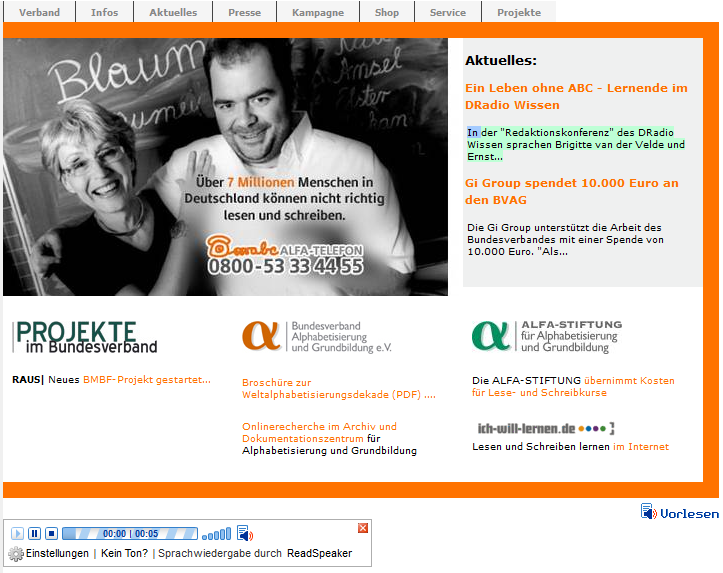
\includegraphics[width=1.00\textwidth]{Daten/DesignBeispiel1.png}
	\caption{Design Beispiel vom Bundesverband Alphabetisierung}
	\label{fig:DesignBeispiel1}
\end{figure}

Hier kann man auf Abb.\ref{fig:DesignBeispiel1} einen markierten Text sehen und unten rechts einen kleinen Button, auf dem "`Vorlesen"' steht. Diese Anwendung ist so gedacht, dass sobald User einen Text markieren, diese den Vorschlag eingeblendet bekommen, dass ihnen dieser Text doch einfach vorgelesen werden könnte. Ohne Zweifel ein Design, dass sich in erster Linie bestenfalls für funktionale Analphabeten auszahlt, oder zumindest für Leute, die eine kurze Einführung erhalten. Jedoch ist die Idee, die hinter dem ganzen steckt eine Fantastische, die dem User eine Möglichkeit anbietet schwierigen Text für ihn zu entziffern, wenn er dazu nicht in der Lage ist. Akkustisch fällt schlimmstenfalls noch das Problem ins Gewicht, dass Worte vielleiht unbekannt sein könnten, aber dies wollen wir hier nicht näher behandeln.\\
Der User kann sich in so wie man es siehr, wirklich jeden Text markieren - ausgenommen natürlich den Text auf Bildern - und ihn sich vorlesen lassen, wodurch er sogar eine Möglichkeit hat, sich die Navigation an der Stirnseite der Seite vorlesen zu lassen. Wenn man also erst einmal weiß, wie man in etwa mit einer Maus umgeht, kann sich jeder User, der dieser Sprache mächtig ist über die ganze Seite navigieren lassen und sich immer anhören, was die Maschine zu sagen hat, wenn er selber es nicht schafft.\\
\newpage
\subsubsection{Reines Text-Design}

Es gibt auch andere Varianten, die reinweg für funktionale Analphabeten gedacht sind. In diesem Punkt kommen wir nun zu der Suchmaschine Invisque (INteractive VIsual Search and QUery Environment). Diese Suchmaschine ist in erster Linie nicht nur für Analphabeten entwickelt worden, aber wurde laut Angaben der Entwickler so weiterentwickelt, dass sie auch für funktionale Analphabeten geeignet sein soll. Um dieses Ziel zu erreichen, haben die Entwickler versucht einigen Problemen, die funktionale Analphabeten haben, entgegen zu wirken, wie das es diesen Menschen schwer fällt sich auf den Text zu konzentrieren, wenn sehr viel ablenkender weiterer Text auf der Seite verteilt wird, oder wenn PopUps auftauchen, oder Werbung allgemein an den Rändern blinkt. All dies blendet Invisque erfolgreich aus mit einer Blanko-Oberfläche. Invisque verwendet einen wenig irritierenden weißen Hintergrund, in den Ecken befinden sich kleine Felder, aus denen man sich weitere Informationen und Navigationsunterstützung besorgen kann. wie auf Abb.\ref{fig:Invisque} zu sehen ist.


\begin{figure}[h]
	\centering
		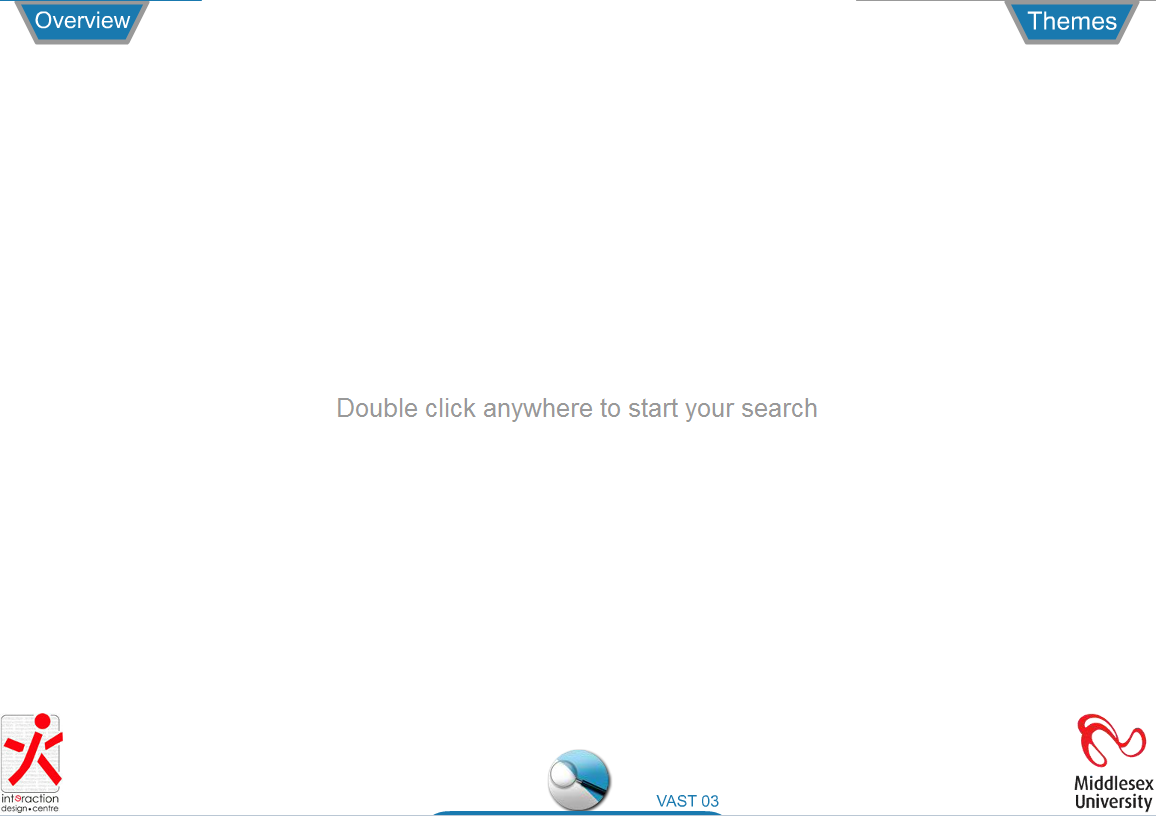
\includegraphics[width=1.00\textwidth]{Daten/Inisque.PNG}
	\caption{Invisque Oberfläche}
	\label{fig:Invisque}
\end{figure}

Um einen guten Überblick über diese suchmaschine zu bekommen, kann man nur empfehlen, es selber ein wenig auszuprobierenund verschiedene Schlüsselwörter einzugeben, mit denen man sich mit der Suche vertraut macht.

\subsubsection{Ein reines Bild Design}

Ein weiterer Ansatz ist es, den Analphabeten ein Interface zu liefern, in dem diese nur über Bilder gezeigt bekommen, worum es geht. Dies ist sicherlich für die Entwicklung eine große Herausforderung, da nicht jeder Mensch Bilder auf die gleiche Weise interpretiert, daher muss darauf geachtet werden, dass die Bilder absolut eindeutig in einem entsprechenden Kontext zugeordnet werden können.\\
Hierbei handelt es sich um eine Anwendung, allen Arten von Analphabeten dabei helfen soll, einen neuen Job zu finden. Diese spezielle Anwendung wurde in Indien entwickelt und speziell für die Menschen dort programmiert. Der Grund und die Inspiration für diese Software war, dass es dort viele Menschen gibt, die wenn sie einen Job haben, diesen nicht mehr aufgeben, auch wenn der Lohn, den sie dafür erhalten viel zu niedrig ist und sie die Chance hätten, einen besseren Job zu bekommen.\\
Das Problem dieser Leute hier, ist was man natürlich an dieser Stelle nicht vergessen darf, dass sie nicht lesen können und entsprechend, nicht über Jobangebote informiert werden. zudem geht es hierbei auch noch um Menschen, die in den Slums wohnen und dadurch besonders wenig Anschluss an die restliche Gesellschaft haben. Daher wollte man diese Software entwickeln um genau diesen Menschen zu helfen, ihre Lebensqualität ein wenig zu verbessern.\\
Um schonmal einen direkten Eindruck von der Applikation zu bekommen, betrachte man bitte Abb.\ref{fig:joblist}.


\begin{figure}[h]
	\centering
		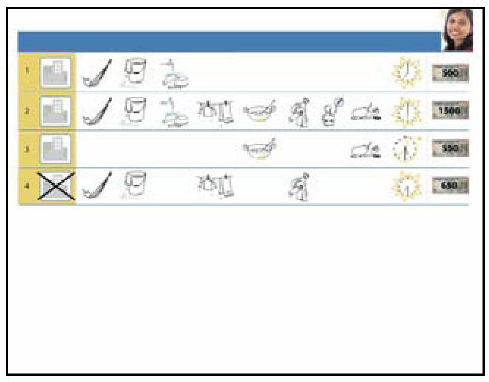
\includegraphics{Daten/job_list.PNG}
	\caption{Job Liste basierend auf Bildern}
	\label{fig:joblist}
\end{figure}

Wie man sieht, besteht die Anwendung wie versprochen nur aus Bildern. Was wir hier sehen, ist eine Liste von Jobs, wobei die Bilder die Beschreibung zu dem liefern, was getan werden soll, wie Fegen oder Kochen. Rechts sind noch eine Uhr abgebildet, die den Menschen sagt, wann sie beginnen müssen zu arbeiten - nähere Informationen, wie wie lange sie arbeiten müssen, erhalten sie, wenn sie diese Job anklicken und damit zu den ausführlicheren Informationen gelangen - und daneben einen Geldschein mit einer Zahl drauf, der ihnen sagt, wieviel sie dort verdienen können.
 
